\documentclass[a4paper,12pt,oneside]{scrreprt}
\usepackage[latin1]{inputenc}
\usepackage[T1]{fontenc}
\usepackage{ae,aecompl}
\usepackage[english]{babel}
\usepackage{amsmath}
\usepackage{amssymb}
\usepackage{amsfonts}
\usepackage{amsthm}
\usepackage{graphicx}
\usepackage{wrapfig}
\usepackage{ulem}
\usepackage{cancel}
\usepackage{float}
\usepackage{color}
\usepackage{titlesec}
\usepackage{geometry}
\geometry{verbose,a4paper,tmargin=25mm,bmargin=25mm,lmargin=15mm,rmargin=25mm}
\titlelabel{\thetitle.\quad}
\usepackage{tabularx}
\usepackage{booktabs}
\usepackage{paralist}
\usepackage{textcomp}

\renewcommand{\rmdefault}{phv}
\renewcommand{\sfdefault}{phv}

\usepackage{listings}
\lstset{
	% numbers=left,
	breaklines=true,
	tabsize=2,
	literate={\ \ }{{\ }}1,
	%	language=C,
	basicstyle=\footnotesize\ttfamily, 
	stepnumber=1,
	%	aboveskip=-10pt,
}


\begin{document}
\begin{tabular}{ccc}
	\begin{large} \textbf{Prof. Lichter} \end{large} &
	
	\begin{minipage}[H]{3.5cm}
	\centering
		\begin{large} OOSC \end{large} \\
		\begin{large} SoSe 2019\end{large}
	\end{minipage} &
	
	\begin{minipage}[H]{4cm}
%		\includegraphics[keepaspectratio,width=\textwidth,angle=0]{logoswc.png}
	\end{minipage} \\
Andreas Steffens, Konrad F\"ogen &  &  \\
& \begin{huge} \textbf{Submission 2} \end{huge}&  \\
& oosc@swc.rwth-aachen.de &  \\
& & \\
 % Hier drunter müssen die Daten noch angepasst werden
%Issued: 1.1.2016 &
%Submission: 1.1.2016 &
%Discussion: 1.1.2016 \\
\end{tabular}
\newline \newline \newline

\begin{center}
	Submitted by Group 09
	
	\bigskip
	
	\begin{tabular}{ll}
		Ulfet CETIN & 391819 \\
		Saud KHAN & 392365  \\
		Samuel ROY & 391822 \\
		Charulekha, Besta Venkateswara RAO & 391844 \\
		Deepak SATEESH & 391813  \\
	\end{tabular}
	
	(ordered on lastname basis)
	
\end{center}


\setcounter{chapter}{1} % Aktuelles Assigment
	
\clearpage


\section{Apply Metrics to a complex software project}
%	\subsection*{b)}
	
	\textbf{java-design-patterns:}
		\begin{compactitem}
			\item McCabe Cyclometric Complexity\\
			
				\begin{center}
					\begin{tabular}{ |c|c|c|c| }
						\hline
						Cyclomatic Complexity & 1.39 & 1.06 & 1.00\\
						\hline
					\end{tabular}
				\end{center}
			
				\begin{figure}[H]
					\centering
					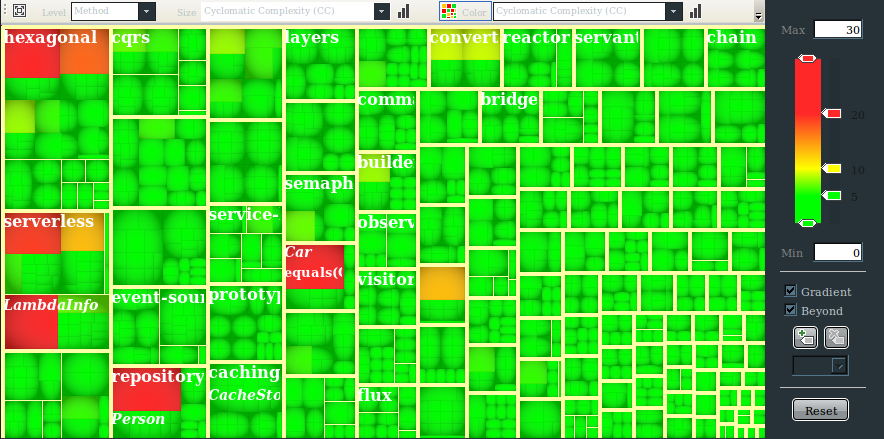
\includegraphics[scale=0.35]{design_cc.png}
					\caption{java-design-patterns - Cyclomatic Complexity (taken using jArchitect)}
				\end{figure}
			
			\item Chidamber \& Kemerer:
			\begin{center}
				\begin{tabular}{ |c|c|c|c| }
					\hline
					Metric Name &  Arithmetic Avg. & StdDev. & Median \\
					\hline
					Number of Methods (per Class) & 1.78 & 1.31 & 1.00\\
					(in place of Weighted Methods per&&&\\
					 Class, as we take system average)&&&\\
					\hline
					Fan-In Visibility (System) & 0.48 & 0.39 & 0.41\\
					(in place of Number of Children -NOC-)&&&\\
					(percentage of internal components in the&&&\\
					 system that depend directly or indirectly &&&\\
					on other components, system-wise)&&&\\
					
					\hline
					Depends Upon (System) & 3.57 & 2.90 & 3.0\\
						Average Component Dependency (ACD) & 2.92 & 1.29 & 2.71\\
					(both in place of Coupling between Objects -CBO-)&&&\\
					\hline
				
					\hline
					Response For a Class (RFC) &&&\\
					(There is no counterpart in SonarGraph)&&&\\
					\hline
					Lack of Cohesion in Methods (LCOM) &&&\\
					(There is no counterpart in SonarGraph)&&&\\
					\hline
				\end{tabular}
			\end{center}
			\bigskip
			\bigskip
			
			\item Robert Martin Metrics:\\
			\begin{center}
				\begin{tabular}{ |c|c|c|c| } 
					\hline
					Metric Name &  Arithmetic Avg. & StdDev. & Median \\
					\hline
					Number of Incoming Dependencies (System) & 0.74 & 1.22 & 0.0\\
					
					Number of Outgoing Dependencies (System) & 0.74 & 1.15 & 0.0\\
					Instability & 0.77 & 0.33 & 1.0 \\
					Abstractness & 0.18 & 0.22 & 0.14 \\
					\hline
				\end{tabular}
			\end{center}
			
			
			
%			\item Metric Suite by Chidamber \& Kemerer
%				\begin{compactitem}
%					\item Weighted Methods per Class (WMC)
%					\item Depth of Inheritance Tree (DIT)
%					\item Number of Children (NOC)
%					\item Coupling between Objects (CBO)
%					\item Response For a Class (RFC)
%					\item Lack of Cohesion in Methods (LCOM)
%				\end{compactitem}
%			
%			\item Robert Martin Metrics
%				\begin{compactitem}
%					\item Efferent Coupling (Ce)
%					\item Afferent Coupling (Ca)
%					\item Instability
%					\item Abstractness
%				\end{compactitem}

	\end{compactitem}
	\bigskip

	* Unless stated otherwise, data is gathered from SonarGraph Explorer.

	
	
	
	
	

\end{document}
